\section{Question 1}

\subsection{The Question}

Demonstrate that you know how to use "curl" well enough to
correctly POST data to a form.  Show that the HTML response that
is returned is "correct".  That is, the server should take the
arguments you POSTed and build a response accordingly.  Save the
HTML response to a file and then view that file in a browser and
take a screen shot.

\subsection{The Answer}

\lstset{
    language=bash,
    label=code:q1_bash,
    caption={Bash script to call cURL}
}

\lstinputlisting{../q1/curlSc.sh}

\lstset{
    language={},
    label=code:q1_test,
    caption={Test file to post on server}
}

\lstinputlisting{../q1/gmicrosTest.txt}


\begin{figure}
\centering
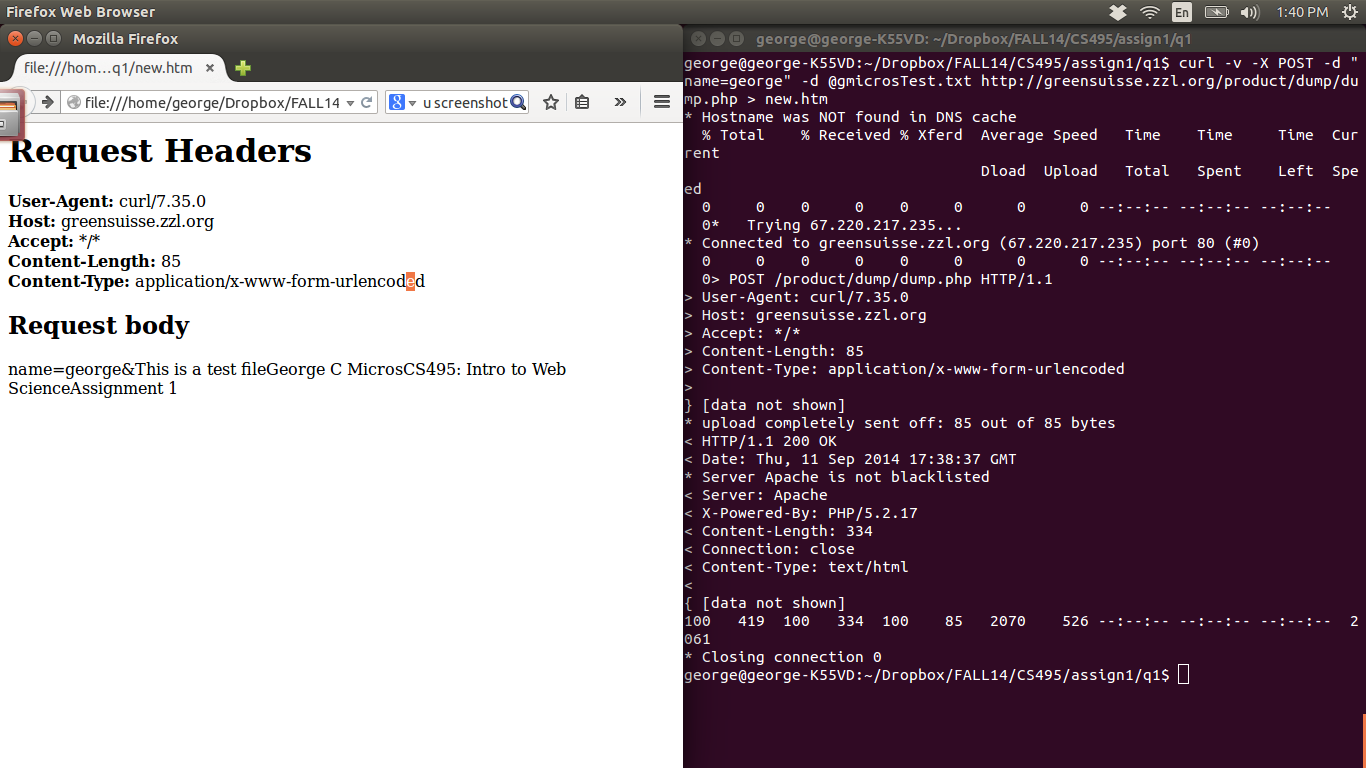
\includegraphics[width=\textwidth]{figures/curlScreen}
\caption{Screenshot of curl request and return}
\end{figure}




